\documentclass{article}
\usepackage{multicol}
\usepackage[utf8]{inputenc}
\usepackage{graphicx}
\usepackage{caption}
\usepackage{subcaption}
\usepackage{float}
\usepackage[a4paper, left=2.5cm, right=2.5cm, top=2.5cm, bottom=2.0cm]{geometry}
\usepackage{url}
\setlength{\parindent}{0pt}
\usepackage[style=IEEE]{biblatex}
\usepackage[symbol]{footmisc}
\usepackage{amsmath, bm}

\newenvironment{Figure}
  {\par\medskip\noindent\minipage{\linewidth}}
  {\endminipage\par\medskip}



\bibliography{MasterThesisPrep}

\begin{document}


\begin{center}
\begin{Large}

Mini review on squaraines
\end{Large}\\
\begin{large}
in preparation of master thesis work\\
\end{large}
\normalsize Maximilian Jeindl\\
\end{center}

\subsection{DOOT}

\begin{multicols}{2}
\section{Structure}
Anilino squaraines, see basic structure in fig. \ref{SQstructureBasic}, have a symmetric structure with an aniline on either side of a squaric acid. The structure electronically is of D-A-D type, with the anilines being donators and the central core being of acceptor type. R here can be either an isobutyl in the case of squaraine with isobutyl sidechains (SQIB) or an alkyl chain of variable length n, leading to for example n-butyl chains as nBSQ or n-octyl chains as nOSQ. \cite{Balzer2022}

\section{Modeling}
\subsection{Kasha theory}

The Kasha model is based entirely on Coulomb coupling between neighboring chromophores, derived from the molecular transition dipole moment interaction. The coupling can be negative or positive (or neutral?) depending on orientation of the aggregates. J-aggregates have negative coupling and are usually associated with relative orientation side-by-side. H-aggregates on the other hand have positive coupling and are orientated head-to-tail.[Introduction]\cite{Hestand2018}
These classifications are based just on coulombic intermolecular coupling within Frenkel exciton theory. Within Frenkel excition theory molecular aggregate photophysics usually use the point-dipole approximation for Coulomb coupling between molecules.\cite{Hestand2018}[Kasha]
\begin{equation}
J=\frac{\boldsymbol{\mu}_1 \cdot \boldsymbol{\mu}_2-3\left(\boldsymbol{\mu}_1 \cdot \hat{R}\right)\left(\boldsymbol{\mu}_2 \cdot \hat{R}\right)}{4 \pi \epsilon R^3}
\end{equation}
Here $\mu$ is the corresponding dipole moment for the $\mathrm{S_0 \rightarrow S_1}$ transition of a molecule. The displacement vectors and the transition dipole moment of the molecules can be simplified by relative positions with an angle $\theta$ between the direction of one transition dipole moment and the relative position vector to the other molecule. At $\theta_{crit} \: = \: 54.7^\circ$ there is no coupling, for smaller angles coupling is negative (J-aggregate) and larger angles positive (H-aggregate).\cite{Hestand2018}[Kasha]
\begin{equation}
J=\frac{\mu^2\left(1-3 \cos ^2 \theta\right)}{4 \pi \varepsilon R^3}
\end{equation}

The Coulomb coupling leads to two delocalized excited states split by 2$|\mathrm{J_C}|$. The in-phase, symmetric, state is shifted by $\mathrm{J_C}$ and the the out-of-phase state is shifted by $-\mathrm{J_C}$. While the in-phase state shows an enhanced transition dipole moment the out-of-phase state is optically dark due to the cancellation of the transition dipole moments. The energy diagram for J and H aggregates can be seen in fig. \cite{Hestand2018}[7073 fig 2]

Additional to the energy shifts of absorption the decay rate is also different for J- an H-aggregates. H-aggregates likely feature a fast intraband relaxation after absorption populating the low energy out-of-phase state, which due to symmetry forbids radiative coupling to the groundstate $|g_1 g_2>$. Meanwhile J-aggregates are radiatively coupled to the groundstate. Compared to the monomer the J-aggregate containing N-coupled molecules has a relaxation enhancement by a factor of N, which is called superradiance. This only concerns radiative decay rate and not total emission yield.\cite{Hestand2018}  

Linear aggregates of N-coupled chromophores with a single molecule per unit cell can be described with the Frenkel exciton hamiltonian in eq. \ref{eq:FrenkelHamilton}, as their delocalized excited states may be described as molecular excitons. There $E_M$ is the monomer $S_0 \rightarrow S_1$ transition energy, D the gas-to-crystal frequency shift, typically negative as neighboring molecules stabilize an excited state via nonresonant interactions, $J_{m,n}$ is the resonant Coulomb coupling between molecules m and n. The states describe a single local excited state ($S_1$) of the $m$th chromophore$|m> \equiv |g_1, g_2, \dots, g_m, \dots, g_N>$.\cite{Hestand2018}

\begin{equation}\label{eq:FrenkelHamilton}
H_{excition} = E_M\:+\:D\:+\sum_{m,n}J_{m,n}|m><n|
\end{equation}

... maybe


Going beyond the point dipole approximation, valid for intermolecular separation lengths larger than the length over which charges separate to produce $\boldsymbol{\mu}$(?). probably \cite{Hestand2018}



\subsection{Alkyl sidechains}
An extended essential states model, based on Painelli's essential states model for DAD chromophores, is used to model the absorption spectra observed. The molecule has two degenerate states, the so called zwitterionic states, due to its symmetry, where the excitation is $\mathrm{D^+A^-D}$ and $\mathrm{DA^-D^+}$ respectively for states $\mathrm{|Z_1>}$ and $\mathrm{|Z_2>}$. The zwitterionic states along with the neutral $\mathrm{|N>}$ DAD together are the essential states model. Compared to the neutral state $\mathrm{|Z_1>}$ and $\mathrm{|Z_2>}$ have a higher energy by $\mu _Z$ and they couple to it through $\mathrm{-t_Z}$.\cite{Balzer2022}


For zwitterionic or ionic states coulombic intermolecular interactions are allowed and vibronic coupling is considered treating the arms as harmonic oscillators. The equilibrium geometry is made dependent on the electronic state. (ref 35) Considering thin films each system is treated as a dimer pair consisting of nearest-neighbor $\pi-$stacked molecules along a axis. \cite{Balzer2022}

\begin{Figure}
\centering
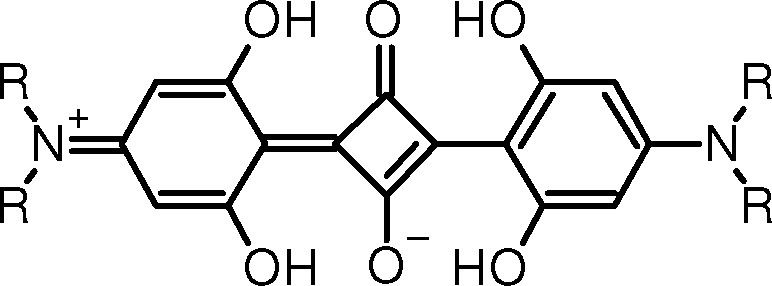
\includegraphics[width = \linewidth]{images/nAlinoSquaraine.jpeg}
\captionof{figure}{asdf\cite{Balzer2022}}
\label{SQstructureBasic}
\end{Figure}

Spin-cast polycristalline nBSQ, nPSQ, nHSQ, nOSQ thin films have polarization a $\lambda \approx 550\: nm\: (\sim 2.25 eV)$ and a $\lambda \approx 650\: nm\: (\sim 1.91 eV)$ peaks. Spectra averaged over crystall directions, thus no polarization dependence observable. $t_\mathrm{CT}$ and $\mu_\mathrm{CT}$ decrease with increasing alkyl chain length. Specifically the trend for $\mu_\mathrm{CT}$ opposes prior publications for nBSQ and nHSQ. In simulations the trend of decreasing $t_\mathrm{CT}$ and $\mu_\mathrm{CT}$ reproduces the relative increase of the high energy peak and the narrowing of the peak spacing. However the high energy peak is wider than the low energy peak from experimental data, whereas the simulation behaves oppositely.\cite{Balzer2022}

Dip coating and drop casting are used to gain larger well ordered but isolated aggregates. Aggregates are several hundred nanometers tall and well isolated. For nHSQ the polarization rotation difference between the absorption peaks in reflection is $|\Delta\Phi^r_{max}| = (7\pm3)^\circ$. For transmission spectroscopy the angle was found to be $|\delta\Phi^{spec}_{max}| = (10 \pm 3)^\circ$. For drop-casting the reflection measurement was reproduced to be the same as $|\Delta\Phi^r_{max}|$ and for transmission $|\delta\Phi^{t}_{max}| = (9 \pm 3)^\circ$. The difference between reflection and transmission measurements are due to polarization rotation within the crystal. The refractive index for nHSQ and nOSQ is ellipsoid, the absorbance ellipsoid is unknown. The same measurements were done for nOSQ microcrystallites form dip coating showing $|\delta\Phi^{spec}_{max}| = (11\pm3)^\circ$, $|\delta\Phi^{t}_{max}| = (12\pm3)^\circ$ and $|\Delta\Phi^r_{max}| = (8\pm3)^\circ$.\cite{Balzer2022}

\begin{table}[H]
\caption{Difference in polarization angles for nHSQ and nOSQ from reflection (r), transmission (t) and spectroscopic transmission (spec) in crystalline samples\cite{Balzer2022}}
\begin{tabular}{l|lll}
compound & $|\delta\Phi^{r}_{max}| [deg]$  & $|\delta\Phi^{t}_{max}| [deg]$  & $|\delta\Phi^{spec}_{max}| [deg]$     \\ \hline
nHSQ     & $7\pm3$ & $9\pm3$  & $10\pm3$ \\
nOSQ     & $8\pm3$ & $12\pm3$ & $11\pm3$
\end{tabular}
\end{table}

The molecular transition dipole is oriented along the long axis of the molecule and the charge-transfer transition dipole is oriented along the $\pi$-stacking axis. \cite{Balzer2022}
The electronic states relevant for absorbance spectra of  squaraine thin films are adequately described as linear combination of neutral and charge separated states $|ge_1>_{AS}$, optically allowed intramolecular exciton, and $|ac_1>_{AS}$, lowest-energy antisymmetric intermolecular charge transfer (ICT) state. Foregoing intermolecular interactions and vibronic coupling they are eigenstates of the system, with $|ge_1>_{AS}$ the having the only nonzero transition dipole moment from the symmetric groundstate $|gg>_S$. \cite{Balzer2022}

Allowing intermolecular charge-transfer inteactions changes ground- and excited- state wavefunctions: $|gg>_S$ mixes  with higher enrgy charge-transfer states leading to a new ground state $|G>_S$ of mixed charge-transfer and neutral character. This results in a transition dipole moment $\mathbf{\mu}^{\left(1\right)}_{CT} \neq 0$ from groundstate to $|ac_1>_{AS}$, allowing for the transition to it. For the nAlkyl systems here $\mathbf{\mu}^{\left(1\right)}_{CT}$ is small relative to the intramolecular $\mathbf{\mu}^{\left(1\right)}_{M}$. Thus the direction of the total dipole is mainly determined by the direction of the intramolecular component. The two polarization peaks come from the two possible combinations of the dipole moments. \cite{Balzer2022}
\newpage

%Going in via the coulomb interaction between molecules in zwitterionic states also leads to the characteristic vibronic spectral features exhibited by J- and H- aggregates from excition theory. For this the charge zwitterionic chargedensities are condensed to pointcharges on the nitrogen atoms and centered in the four-membered ring.\cite{Hestand2015}
\section{Measurements}
\subsection{SQIB}
\subsection{nAlkyl}


\newpage
\printbibliography
\end{multicols}


\end{document}




